\documentclass[12pt,a4paper]{article}
\usepackage[utf8]{inputenc}
\usepackage[T1]{fontenc}
\usepackage{geometry}
\usepackage{amsmath, amssymb}
\usepackage{listings}
\usepackage{xcolor}
\usepackage{booktabs}
\usepackage{array}
\usepackage{hyperref}
\usepackage{tikz}
\usetikzlibrary{positioning, arrows.meta}

\geometry{left=2.5cm, right=2.5cm, top=2.5cm, bottom=2.5cm}

\definecolor{codebg}{rgb}{0.96,0.96,0.96}
\definecolor{codegreen}{rgb}{0.0,0.5,0.0}
\definecolor{codegray}{rgb}{0.5,0.5,0.5}
\definecolor{codepurple}{rgb}{0.58,0,0.82}
\definecolor{codeblue}{rgb}{0.0,0.0,0.8}

\lstdefinestyle{javastyle}{
    backgroundcolor=\color{codebg},
    commentstyle=\color{codegreen}\itshape,
    keywordstyle=\color{codeblue}\bfseries,
    stringstyle=\color{codepurple},
    numberstyle=\tiny\color{codegray},
    basicstyle=\ttfamily\small,
    breaklines=true,
    keepspaces=true,
    numbers=left,
    numbersep=5pt,
    language=Java,
    frame=single,
    rulecolor=\color{codegray}
}

\hypersetup{colorlinks=true, linkcolor=blue, urlcolor=cyan}

\title{
    \Huge \textbf{Minimum Spanning Tree} \\[0.5em]
    \Large Prim's \& Kruskal's Algorithms \\[0.5em]
    \large Data Structures \& Algorithms Reference
}
\author{Algorithm Study Guide}
\date{\today}

\begin{document}

\maketitle
\tableofcontents
\newpage

% ============================================================
\section{Introduction}
% ============================================================

\subsection{What is a Spanning Tree?}
Given a connected, undirected graph $G = (V, E)$, a \textbf{spanning tree} $T$ is a subgraph that:
\begin{itemize}
    \item Includes \textbf{all} $V$ vertices of $G$.
    \item Is a \textbf{tree} (connected + acyclic).
    \item Contains exactly $V - 1$ edges.
\end{itemize}

\subsection{What is a Minimum Spanning Tree?}
A \textbf{Minimum Spanning Tree (MST)} is a spanning tree whose total edge weight is \textbf{minimized}:
\[
\text{MST} = \arg\min_{T \text{ spanning tree}} \sum_{(u,v) \in T} w(u,v)
\]
A graph may have multiple MSTs (if edge weights are not all distinct), but they all have the same total weight.

\subsection{Key Properties}
\begin{enumerate}
    \item \textbf{Cut Property}: For any cut $(S, V \setminus S)$ of $G$, the minimum-weight edge crossing the cut belongs to some MST.
    \item \textbf{Cycle Property}: The maximum-weight edge in any cycle of $G$ does \textit{not} belong to any MST.
\end{enumerate}
Both Prim's and Kruskal's algorithms rely on these greedy properties.

\subsection{Complexity Comparison}
\begin{table}[h!]
\centering
\renewcommand{\arraystretch}{1.4}
\begin{tabular}{|l|c|c|l|}
\hline
\textbf{Algorithm} & \textbf{Time} & \textbf{Space} & \textbf{Best For} \\
\hline
Prim's (Min-Heap)  & $O(E \log V)$ & $O(V + E)$     & Dense graphs \\
Kruskal's          & $O(E \log E)$ & $O(V + E)$     & Sparse graphs \\
\hline
\end{tabular}
\caption{$V$ = vertices, $E$ = edges}
\end{table}

\subsection{Applications}
\begin{itemize}
    \item \textbf{Network design}: Laying cables, roads, or pipelines with minimum cost.
    \item \textbf{Cluster analysis}: Grouping similar data points.
    \item \textbf{Image segmentation}: Partition pixels into regions.
    \item \textbf{Approximation algorithms}: 2-approximation for Metric TSP.
    \item \textbf{Circuit design}: Minimising wire length on a PCB.
\end{itemize}

\newpage

% ============================================================
\section{Prim's Algorithm}
% ============================================================

\subsection{Concept}
Prim's is a \textbf{greedy algorithm} that \textbf{grows the MST one vertex at a time}. Starting from an arbitrary vertex, it repeatedly adds the minimum-weight edge connecting a vertex already in the MST to one not yet in it.

\subsection{Algorithm Steps}
\begin{enumerate}
    \item Initialize: $\text{key}[v] = \infty$ for all $v$; $\text{key}[\text{src}] = 0$.
    \item Insert all vertices into a \textbf{Min-Heap} (Priority Queue) keyed by $\text{key}[v]$.
    \item While Min-Heap is not empty:
    \begin{enumerate}
        \item Extract vertex $u$ with minimum $\text{key}[u]$. Add $u$ to MST.
        \item For each neighbor $v$ of $u$ not yet in MST:
        \[
            \text{if } w(u,v) < \text{key}[v]: \quad \text{key}[v] \leftarrow w(u,v),\; \text{parent}[v] \leftarrow u
        \]
        \item Update $v$ in the Min-Heap.
    \end{enumerate}
\end{enumerate}

\subsection{Example}

Consider the following weighted graph:
\begin{center}
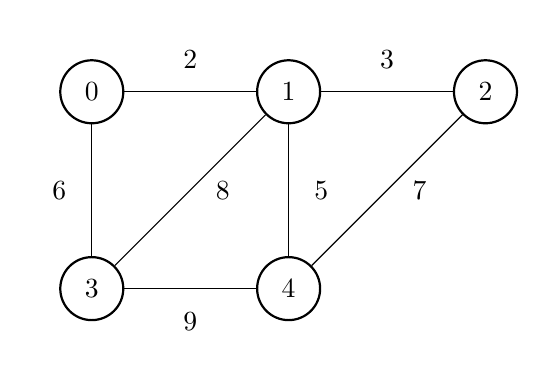
\begin{tikzpicture}[
    node distance=2.5cm,
    every node/.style={circle, draw, thick, minimum size=0.8cm},
    every edge/.style={draw, thick}
]
\node (0) {0};
\node (1) [right of=0] {1};
\node (2) [right of=1] {2};
\node (3) [below of=0] {3};
\node (4) [below of=1] {4};

\draw (0) -- node[above,draw=none] {2} (1);
\draw (1) -- node[above,draw=none] {3} (2);
\draw (0) -- node[left, draw=none] {6} (3);
\draw (1) -- node[right,draw=none] {8} (3);
\draw (1) -- node[right,draw=none] {5} (4);
\draw (2) -- node[right,draw=none] {7} (4);
\draw (3) -- node[below,draw=none] {9} (4);
\end{tikzpicture}
\end{center}

\textbf{MST edges} (starting from vertex 0): $(0,1,2),\; (1,2,3),\; (1,4,5),\; (0,3,6)$

\textbf{Total MST weight} $= 2 + 3 + 5 + 6 = 16$

\subsection{Java Implementation}
\begin{lstlisting}[style=javastyle, caption={Prim's Algorithm — Java}]
public static void primsAlgorithm(int[][] graph, int V) {
    int[] key    = new int[V];   // min weight to reach each vertex
    int[] parent = new int[V];   // MST parent of each vertex
    boolean[] inMST = new boolean[V];
    Arrays.fill(key, Integer.MAX_VALUE);
    Arrays.fill(parent, -1);
    key[0] = 0;

    // Min-Heap: {key, vertex}
    PriorityQueue<int[]> pq =
        new PriorityQueue<>(Comparator.comparingInt(a -> a[0]));
    pq.offer(new int[]{0, 0});

    while (!pq.isEmpty()) {
        int u = pq.poll()[1];
        if (inMST[u]) continue;
        inMST[u] = true;

        for (int v = 0; v < V; v++) {
            if (graph[u][v] != 0 && !inMST[v]
                    && graph[u][v] < key[v]) {
                key[v]    = graph[u][v];
                parent[v] = u;
                pq.offer(new int[]{key[v], v});
            }
        }
    }
}
\end{lstlisting}

\subsection{Complexity}
\begin{itemize}
    \item \textbf{Time}: $O(E \log V)$ with adjacency list + Min-Heap.
    \item \textbf{Space}: $O(V)$ for key/parent/inMST arrays + heap.
    \item \textbf{Greedy Proof}: Follows the \textit{Cut Property} — always picks the minimum cross-cut edge.
\end{itemize}

\newpage

% ============================================================
\section{Kruskal's Algorithm}
% ============================================================

\subsection{Concept}
Kruskal's is a \textbf{greedy algorithm} that sorts all edges by weight and adds them to the MST \textbf{one by one}, skipping any edge that would create a cycle. Cycle detection is done efficiently with a \textbf{Disjoint Set Union (DSU)} structure.

\subsection{Algorithm Steps}
\begin{enumerate}
    \item Sort all $E$ edges in ascending order of weight.
    \item Initialize DSU: each vertex is its own component.
    \item For each edge $(u, v, w)$ in sorted order:
    \begin{enumerate}
        \item If $\text{find}(u) \ne \text{find}(v)$: add edge to MST; $\text{union}(u, v)$.
        \item Else: skip (adding this edge would form a cycle).
    \end{enumerate}
    \item Stop when MST has $V - 1$ edges.
\end{enumerate}

\subsection{Disjoint Set Union (DSU)}
DSU (also called Union-Find) maintains a forest of trees. Two optimizations make it near-constant time:
\begin{itemize}
    \item \textbf{Path Compression}: During \texttt{find}, make every node point directly to its root.
    \item \textbf{Union by Rank}: Always attach the shorter tree under the taller one.
\end{itemize}
With both optimizations: $O(\alpha(V)) \approx O(1)$ per operation (inverse Ackermann function).

\subsection{Java Implementation}
\begin{lstlisting}[style=javastyle, caption={Kruskal's Algorithm with DSU — Java}]
public static void kruskalsAlgorithm(int V, List<Edge> edges) {
    Collections.sort(edges);  // Sort by weight
    int[] parent = new int[V];
    int[] rank   = new int[V];
    for (int i = 0; i < V; i++) parent[i] = i;  // each is its own root

    List<Edge> mst = new ArrayList<>();
    for (Edge edge : edges) {
        int rootU = find(parent, edge.src);
        int rootV = find(parent, edge.dest);
        if (rootU != rootV) {            // different components -> no cycle
            mst.add(edge);
            union(parent, rank, rootU, rootV);
            if (mst.size() == V - 1) break;
        }
    }
}

// Path-compression find
private static int find(int[] parent, int x) {
    if (parent[x] != x)
        parent[x] = find(parent, parent[x]);
    return parent[x];
}

// Union by rank
private static void union(int[] parent, int[] rank, int x, int y) {
    if (rank[x] < rank[y])       parent[x] = y;
    else if (rank[x] > rank[y])  parent[y] = x;
    else { parent[y] = x; rank[x]++; }
}
\end{lstlisting}

\subsection{Complexity}
\begin{itemize}
    \item \textbf{Sorting}: $O(E \log E)$
    \item \textbf{DSU operations}: $O(E \cdot \alpha(V)) \approx O(E)$
    \item \textbf{Total}: $O(E \log E)$
    \item \textbf{Greedy Proof}: Follows the \textit{Cycle Property} — never adds the maximum edge of any cycle.
\end{itemize}

\newpage

% ============================================================
\section{Prim's vs Kruskal's}
% ============================================================

\begin{table}[h!]
\centering
\renewcommand{\arraystretch}{1.5}
\begin{tabular}{|l|p{5.5cm}|p{5.5cm}|}
\hline
\textbf{Property}      & \textbf{Prim's}                    & \textbf{Kruskal's}                \\
\hline
Strategy               & Grow MST vertex by vertex           & Add minimum edges globally        \\
Data Structure         & Min-Heap (Priority Queue)           & Sort + DSU (Union-Find)           \\
Time Complexity        & $O(E \log V)$                      & $O(E \log E)$                     \\
Best For               & Dense graphs                        & Sparse graphs                     \\
Greedy Rule            & Cut Property                        & Cycle Property                    \\
Implementation         & More complex (priority queue)       & Simpler (sort + union-find)       \\
Graph Type             & Connected graph                     & Can detect forests                \\
\hline
\end{tabular}
\caption{Prim's vs Kruskal's Comparison}
\end{table}

\section{Key Formulas}

\begin{align}
\text{Spanning tree edges:}\quad      & |E_{\text{MST}}| = V - 1 \\
\text{Prim's complexity:}\quad        & T = O(E \log V) \\
\text{Kruskal's complexity:}\quad     & T = O(E \log E) \\
\text{DSU find/union (amortised):}\quad & T = O(\alpha(V)) \approx O(1) \\
\text{Cut Property:}\quad             & \min\text{-edge crossing any cut} \in \text{some MST} \\
\text{Cycle Property:}\quad           & \max\text{-edge of any cycle} \notin \text{any MST}
\end{align}

\end{document}
